% ============================================================
%  SCHOLA DOMESTICA — Level 1, Week 1, Lesson 2
%  Topic: Number 3
% ============================================================
\documentclass[12pt,letterpaper]{article}
\usepackage[top=1in,bottom=1in,left=1in,right=1in]{geometry}
\usepackage{fontspec}\usepackage{graphicx}\usepackage{xcolor}
\usepackage{mdframed}\usepackage{tikz}\usepackage{fancyhdr}\usepackage{parskip}
\usetikzlibrary{shapes.geometric}
\setmainfont{EB Garamond}[Ligatures=TeX,Numbers=OldStyle]
\definecolor{sd-blue}{RGB}{60,100,160}\definecolor{sd-gold}{RGB}{180,140,50}
\definecolor{sd-light}{RGB}{245,242,235}\definecolor{sd-green}{RGB}{70,130,80}
\pagestyle{fancy}\fancyhf{}
\fancyhead[L]{\small\color{sd-blue}\textit{Schola Domestica Mathematics}}
\fancyhead[R]{\small\color{sd-blue}\textit{Level~1 \(\cdot\) Week~1 \(\cdot\) Lesson~2}}
\fancyfoot[C]{\small\color{sd-blue}1}
\renewcommand{\headrulewidth}{0.4pt}
\newmdenv[backgroundcolor=sd-light,linecolor=sd-blue,linewidth=1pt,
  innerleftmargin=10pt,innerrightmargin=10pt,innertopmargin=8pt,
  innerbottommargin=8pt,roundcorner=4pt]{instructbox}
\newmdenv[backgroundcolor=white,linecolor=sd-green,linewidth=1.5pt,
  innerleftmargin=10pt,innerrightmargin=10pt,innertopmargin=8pt,
  innerbottommargin=8pt,roundcorner=4pt]{checkbox}
\newcommand{\ansblank}{\underline{\hspace{1.6cm}}}
\newcounter{probnum}
\newcommand{\prob}{\stepcounter{probnum}\noindent\textbf{\arabic{probnum}.}\quad}
\newcommand{\onestar}{
\begin{tikzpicture}[baseline=-0.1cm]
  \node[star,star points=5,star point ratio=2.5,fill=sd-gold,
        draw=sd-gold!80!black,minimum size=0.9cm]{};
  \end{tikzpicture}}
\begin{document}
\begin{center}
  {\color{sd-blue}\Large\bfseries Schola Domestica Mathematics — Level~1}\\[4pt]
  {\color{sd-blue}\rule{\linewidth}{1.5pt}}\\[6pt]
  {\LARGE\bfseries Lesson 2 \quad|\quad The Number 3}\\[4pt]
  {\color{sd-gold}\rule{\linewidth}{0.8pt}}
\end{center}
\vspace{4pt}
\begin{instructbox}
\noindent\textbf{\color{sd-blue}Instruction:}\\[4pt]
Today we learn the number \textbf{3}.
Count with me: one, two, three.
Three is one more than two.
\end{instructbox}
\vspace{8pt}
\noindent\textbf{\color{sd-blue}Trace and write:}
\vspace{4pt}
\begin{center}
\begin{tabular}{|c|c|c|c|c|}
\hline
\rule{0pt}{26pt}{\Huge\color{sd-blue!40}3}&{\Huge\phantom{3}}&{\Huge\phantom{3}}&{\Huge\phantom{3}}&{\Huge\phantom{3}}\\
\hline
\end{tabular}
\end{center}
\vspace{6pt}{\color{sd-gold}\rule{\linewidth}{0.5pt}}\vspace{6pt}
\noindent\textbf{\color{sd-blue}Practice}
\vspace{4pt}

\prob Count the ducks. How many? \quad
\IfFileExists{ducks_3.jpg}{
\includegraphics[height=1.4cm]{ducks_3.jpg}}{%
  
\begin{tikzpicture}[baseline=0]
    \foreach \x in {0,1,2} \draw[fill=yellow!70,thick](\x*0.9,0)ellipse(0.35 and 0.25);
  \end{tikzpicture}}
\quad\ansblank

\vspace{8pt}
\prob Count the stars.\quad\onestar\quad\onestar\quad\onestar\quad\ansblank

\vspace{8pt}
\prob Circle the group of \textbf{3}:
\vspace{4pt}
\begin{center}
\begin{tabular}{ccccc}
{\large\textbf{A}}\quad\onestar\onestar &\quad\quad&
{\large\textbf{B}}\quad\onestar\onestar\onestar &\quad\quad&
{\large\textbf{C}}\quad\onestar
\end{tabular}
\end{center}

\vspace{8pt}
\prob Draw \textbf{3} circles:
\vspace{2pt}
\noindent\fbox{\rule{0pt}{2cm}\hspace{9cm}}

\vspace{8pt}
\prob \textit{(Teacher reads)} A mouse found 1~acorn, then 1~more, then 1~more.
How many acorns does the mouse have? \quad\ansblank

\vspace{8pt}
\prob How many? \quad
\IfFileExists{apples_3.jpg}{
\includegraphics[height=1.4cm]{apples_3.jpg}}{%
  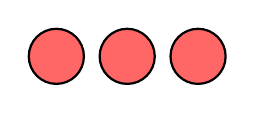
\begin{tikzpicture}[baseline=0]
    \foreach \x in {0,1,2}\draw[fill=red!60,thick](\x*0.9,0)circle(0.35);
  \end{tikzpicture}}
\quad\ansblank

\vspace{8pt}
\prob Write the number that comes after 2: \quad\ansblank

\vspace{8pt}
\prob Put the numbers in order from smallest to biggest:\\[4pt]
\hspace{2cm}{\Large 3 \quad 1 \quad 2} \quad $\longrightarrow$ \quad
\ansblank \quad \ansblank \quad \ansblank

\vspace{8pt}{\color{sd-gold}\rule{\linewidth}{0.5pt}}\vspace{4pt}
\begin{checkbox}
\noindent\textbf{\color{sd-green}Knowledge Check}\\[4pt]
\setcounter{probnum}{0}
\prob How many? \quad\onestar\onestar\onestar\quad\ansblank\\[8pt]
\prob Write the number 3: \quad\ansblank
\end{checkbox}
\vfill
\noindent{\color{sd-blue}$\bigstar$ \textbf{Enrichment:}}
In Latin, three is \textit{tr\={e}s}.
Count to three in Latin: \textit{ūnus, duo, tr\={e}s}!
\vspace{4pt}\hrule\vspace{2pt}
{\footnotesize\color{gray}\textit{Teacher note: Ask student to find three objects in the room.}}
\end{document}

% ============================================================
%  END LESSON 2
% ============================================================
